
\graphicspath{ {mainmatter/Birnbaum_2005/} }
\title*{2005: Towards a Dimension Space for Musical Devices}
\titlerunning{Dimension Space for Musical Devices}

\author{David Birnbaum, Rebecca Fiebrink, Joseph Malloch, and Marcelo M. Wanderley}
\authorrunning{Birnbaum et al.}

%\institute{David Birnbaum \at Immersion Corporation, 50 Rio Robles, San Jose, CA, 94607, USA, \email{davidmbirnbaum@gmail.com}
%\and Rebecca Fiebrink \at Goldsmiths, University of London, London, SE14 6NW, UK, \email{r.fiebrink@gold.ac.uk}
%\and Joseph Malloch \at ExSitu, Inria, Universit\'{e} Paris-Saclay and LRI, Universit\'{e} Paris-Sud, CNRS, Universit\'{e} Paris-Saclay, 91405, Orsay, France, \email{joseph.malloch@inria.fr}
%\and Marcelo M. Wanderley \at Input Devices and Music Interaction Laboratory (IDMIL), Centre for Interdisciplinary Research in Music Media and Technology (CIRMMT), McGill University, 555 Sherbrooke Street West, H3A 1E3 Montreal, Qc, Canada, \email{marcelo.wanderley@mcgill.ca}}
%
% Use the package ''url.sty'' to avoid
% problems with special characters
% used in your e-mail or web address
%
\maketitle

\abstract*{While several researchers have grappled with the problem of comparing musical devices across performance, installation, and related contexts, no methodology yet exists for producing holistic, informative visualizations for these devices. Drawing on existing research in performance interaction, human-computer interaction, and design space analysis, the authors propose a dimension space representation that can be adapted for visually displaying musical devices. This paper illustrates one possible application of the dimension space to existing performance and interaction systems, revealing its usefulness both in exposing patterns across existing musical devices and aiding in the design of new ones.}

\section{Examining Musical Devices}

Musical devices can take varied forms, including interactive installations, digital musical instruments, and augmented instruments. Trying to make sense of this wide variability, several researchers have proposed frameworks for classifying the various systems.

As early as 1985, Pennycook \cite{Pennycook:1985} offered a discussion of interface concepts and design issues. Pressing \cite{Pressing:1990} proposed a set of fundamental design principles for computer-music interfaces. His exhaustive treatment of the topic laid the groundwork for further research on device characterization.

Bongers \cite{Bongers:2000} characterized musical interactions as belonging to one of three modes: Performer--System interaction, such as a performer playing an instrument, System--Audience interaction, such as those commonly found at interactive sound installations, and Performer--System--Audience interaction, which describes interactive systems in which both artist and audience interact in real time.

 \cite{Wanderley:2000} discussed two approaches to classification of musical devices, including instruments and installations: the technological perspective and the semantical perspective. \cite{Ulyate:2001} characterizes instruments in terms of music output complexity, control input complexity and performer freedom. Focusing on interactive installations, Winkler \cite{Winkler:2000} discussed digital, physical, social, and personal factors that should be considered in their design. In a similar way, Blaine and Fels \cite{Blaine:2003a} studied design features of collaborative musical systems, with the particular goal of elucidating design issues endemic to systems for novice players.

While these various approaches contribute insight to the problem of musical device classification, most did not provide a visual representation, which could facilitate device comparison and design. One exception is \cite{Wanderley:2000}, who proposed a basic visualization employing two axes: type of user action and user expertise (Figure~\ref{Birnbaum:fig:wanderley}). Piringer \cite{Piringer:2001} offers a more developed representation, as shown in Figure~\ref{Birnbaum:fig:piringer}. However, both of these representations are limited to only a few dimensions. Furthermore, the configurations could be misread to imply orthogonality of the dimensions represented by the x- and y-axes.

\begin{figure}[t]
\centering
\centering
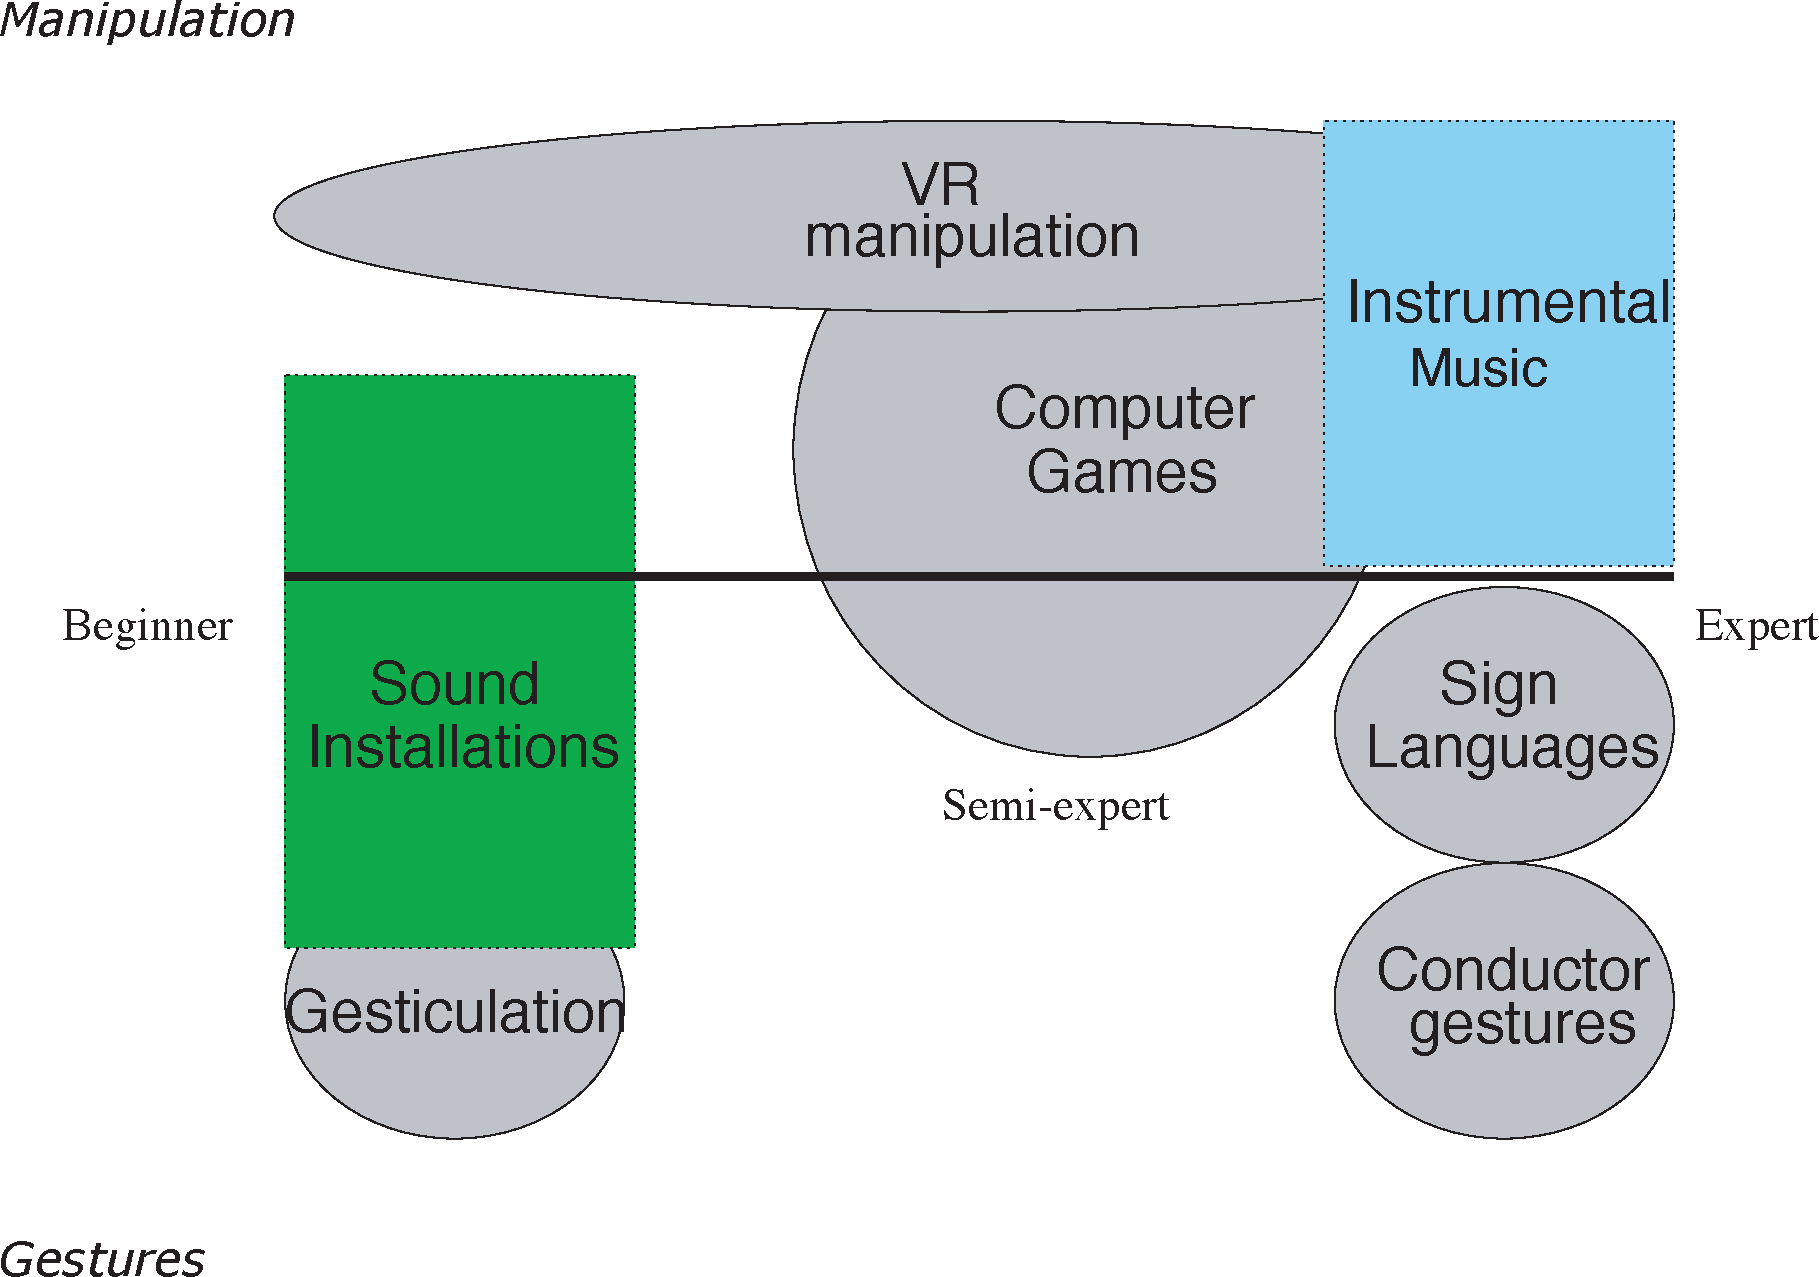
\includegraphics[width=\columnwidth]{figures/wanderley_et_al}
\caption{The 2-dimensional representation of Wanderley et al. \cite{Wanderley:2000}}
\label{Birnbaum:fig:wanderley}
\end{figure}

\begin{figure}[t]
\centering
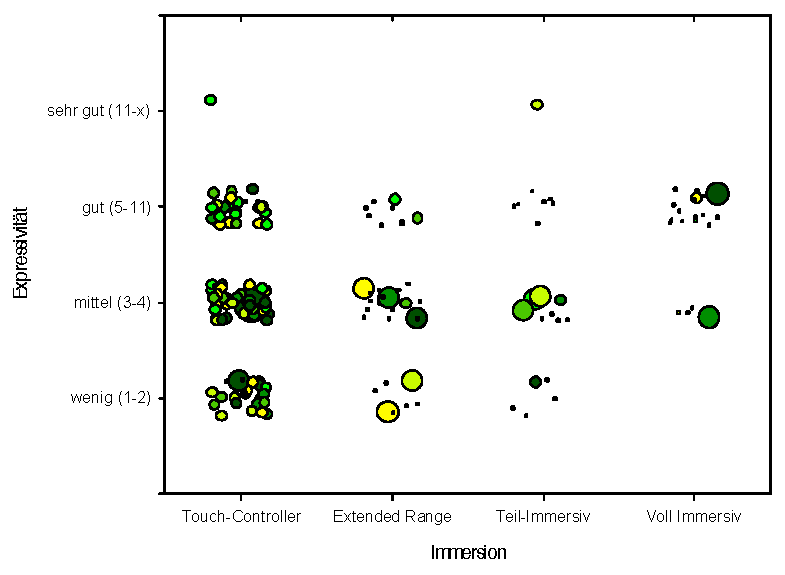
\includegraphics[width=\columnwidth]{figures/piringer}
\caption{An example of a visual representation by Piringer \cite{Piringer:2001}. ``Expressivity'' appears on the y-axis, with the categories \emph{very good}, \emph{good}, \emph{middle}, and \emph{very little} (top to bottom). ``Immersion'' appears on the x-axis, with the categories \emph{Touch-Controller}, \emph{Extended-Range}, \emph{Partially Immersive}, and \emph{Fully Immersive}, and adaptation from \cite{Mulder:1998}. Each shape represents an instrument; the size indicates the amount of feedback and the color indicates feedback modality.}
\label{Birnbaum:fig:piringer}
\end{figure}

The goal of this text is to illustrate an efficient, visually-oriented approach to label{Birnbaum:ing, discussing, and evaluating a broad range of musical systems. Musical contexts where these systems could be of potential interest might relate to \emph{Instrumental manipulation} (e.g., \cite{Waisvisz:1985}), \emph{Control of pre-recorded sequences of events} (see \cite{Mathews:1989,Boie:1989b}), \emph{Control of sound diffusion in multi-channel sound environments}, \emph{Interaction in the context of (interactive) multimedia installations} ( \cite{Winkler:2000}, for example), \emph{Interaction in dance-music systems} \cite{Camurri:1995}, and \emph{Interaction in computer game systems}. Systems in this diverse set involve a range of demands on the user(s) that characterize the human-system interaction, and these demands can be studied with a focus on the underlying system designs. The HCI-driven approach chosen for this study is \emph{design space analysis}.

\section{Design Space Analysis}

Initially proposed as a tool for software design in \cite{MacLean:1993} and \cite{MacLean:1995}, design space analysis offers tools for examining a system in terms of a general framework of theoretical and practical design decisions. Through formal application of ``QOC'' analysis comprised of \emph{Questions} about design, \emph{Options} of how to address these questions, and \emph{Criteria} regarding the suitability of the available options, one generates a visual representation of the ``design space'' of a system. In effect, this representation distinguishes the design rationale behind a system from the set of all possible design decisions. MacLean \cite{MacLean:1993} outlines two goals of the design space analysis approach: to ``develop a technique for representing design decisions which will, even on its own, support and augment design practice,'' and to ``use the framework as a vehicle for communicating and contextualising more analytic approaches to usersystem [sic] interaction into the practicalities of design.''

\subsection{Dimension Space Analysis}

\emph{Dimension space analysis} is a related approach to system design that retains the goals of supporting design practice and facilitating communication \cite{Graham:2000}. Although dimension space analysis does not explicitly incorporate the QOC method of outlining the design space of a system, it preserves the notion of a system inhabiting a finite space within the space of all possible design options, and it sets up the dimensions of this space to correspond to various object properties.

The Dimension Space outlined  by Graham \cite{Graham:2000} represents interactive systems on six axes. Each system component is plotted as a separate dimension space so that the system can be examined from several points of view. Some axes represent a \emph{continuum} from one extreme to another, such as the \emph{Output Capacity} axis, whose values range from \emph{low} to \emph{high}. Others contain only a few \emph{discrete points} in logical progression, such as \emph{Attention Received}, which contains the points \emph{high}, \emph{peripheral}, and \emph{none}. The \emph{Role} axis is the most eccentric, containing five unordered points.

A dimension plot is generated by placing points on each axis, and connecting them to form a two-dimensional shape. They are created from the perspective of a specific entity involved in the interaction. Systems and their components can then be compared rapidly by comparing their respective plots. The shape of the individual plots, however, contain no intended meaning.

The flexibility of the dimension space approach lies in the ability to redefine the axes. In adapting this method, the choice of axes and their possible values is made with respect to the range of systems being considered, and the significant features to be used to distinguish among them. Plotting a system onto a Dimension Space is an exercise that forces the designer to examine each of its characteristics individually, and it exposes important issues that may arise during the design or use of a system.

We illustrate one possible adaptation of \cite{Graham:2000}'s multi-axis graph to classify and plot musical devices ranging from digital musical instruments to sound installations. For this exercise, we chose axes that would meaningfully display design differences among devices, and plotted each device only once, rather than creating multiple plots from different perspectives.

\subsection{An Example Dimension Space}

In adapting the dimension space to the analysis of musical devices, we explored several quantities and configurations of axes. It was subjectively determined that the functionality of the spaces was not affected in plots with as many as eight axes. As an example, Figure~\ref{Birnbaum:fig:7axes} shows a seven-axis configuration, label{Birnbaum:ed with representative ranges. Figure~\ref{Birnbaum:fig:plots} shows plots of several devices, drawn from the areas of digital musical instruments and interactive installations incorporating sound and/or music. Each of the axes are described in detail in the following section.

\begin{figure}[t]
\centering
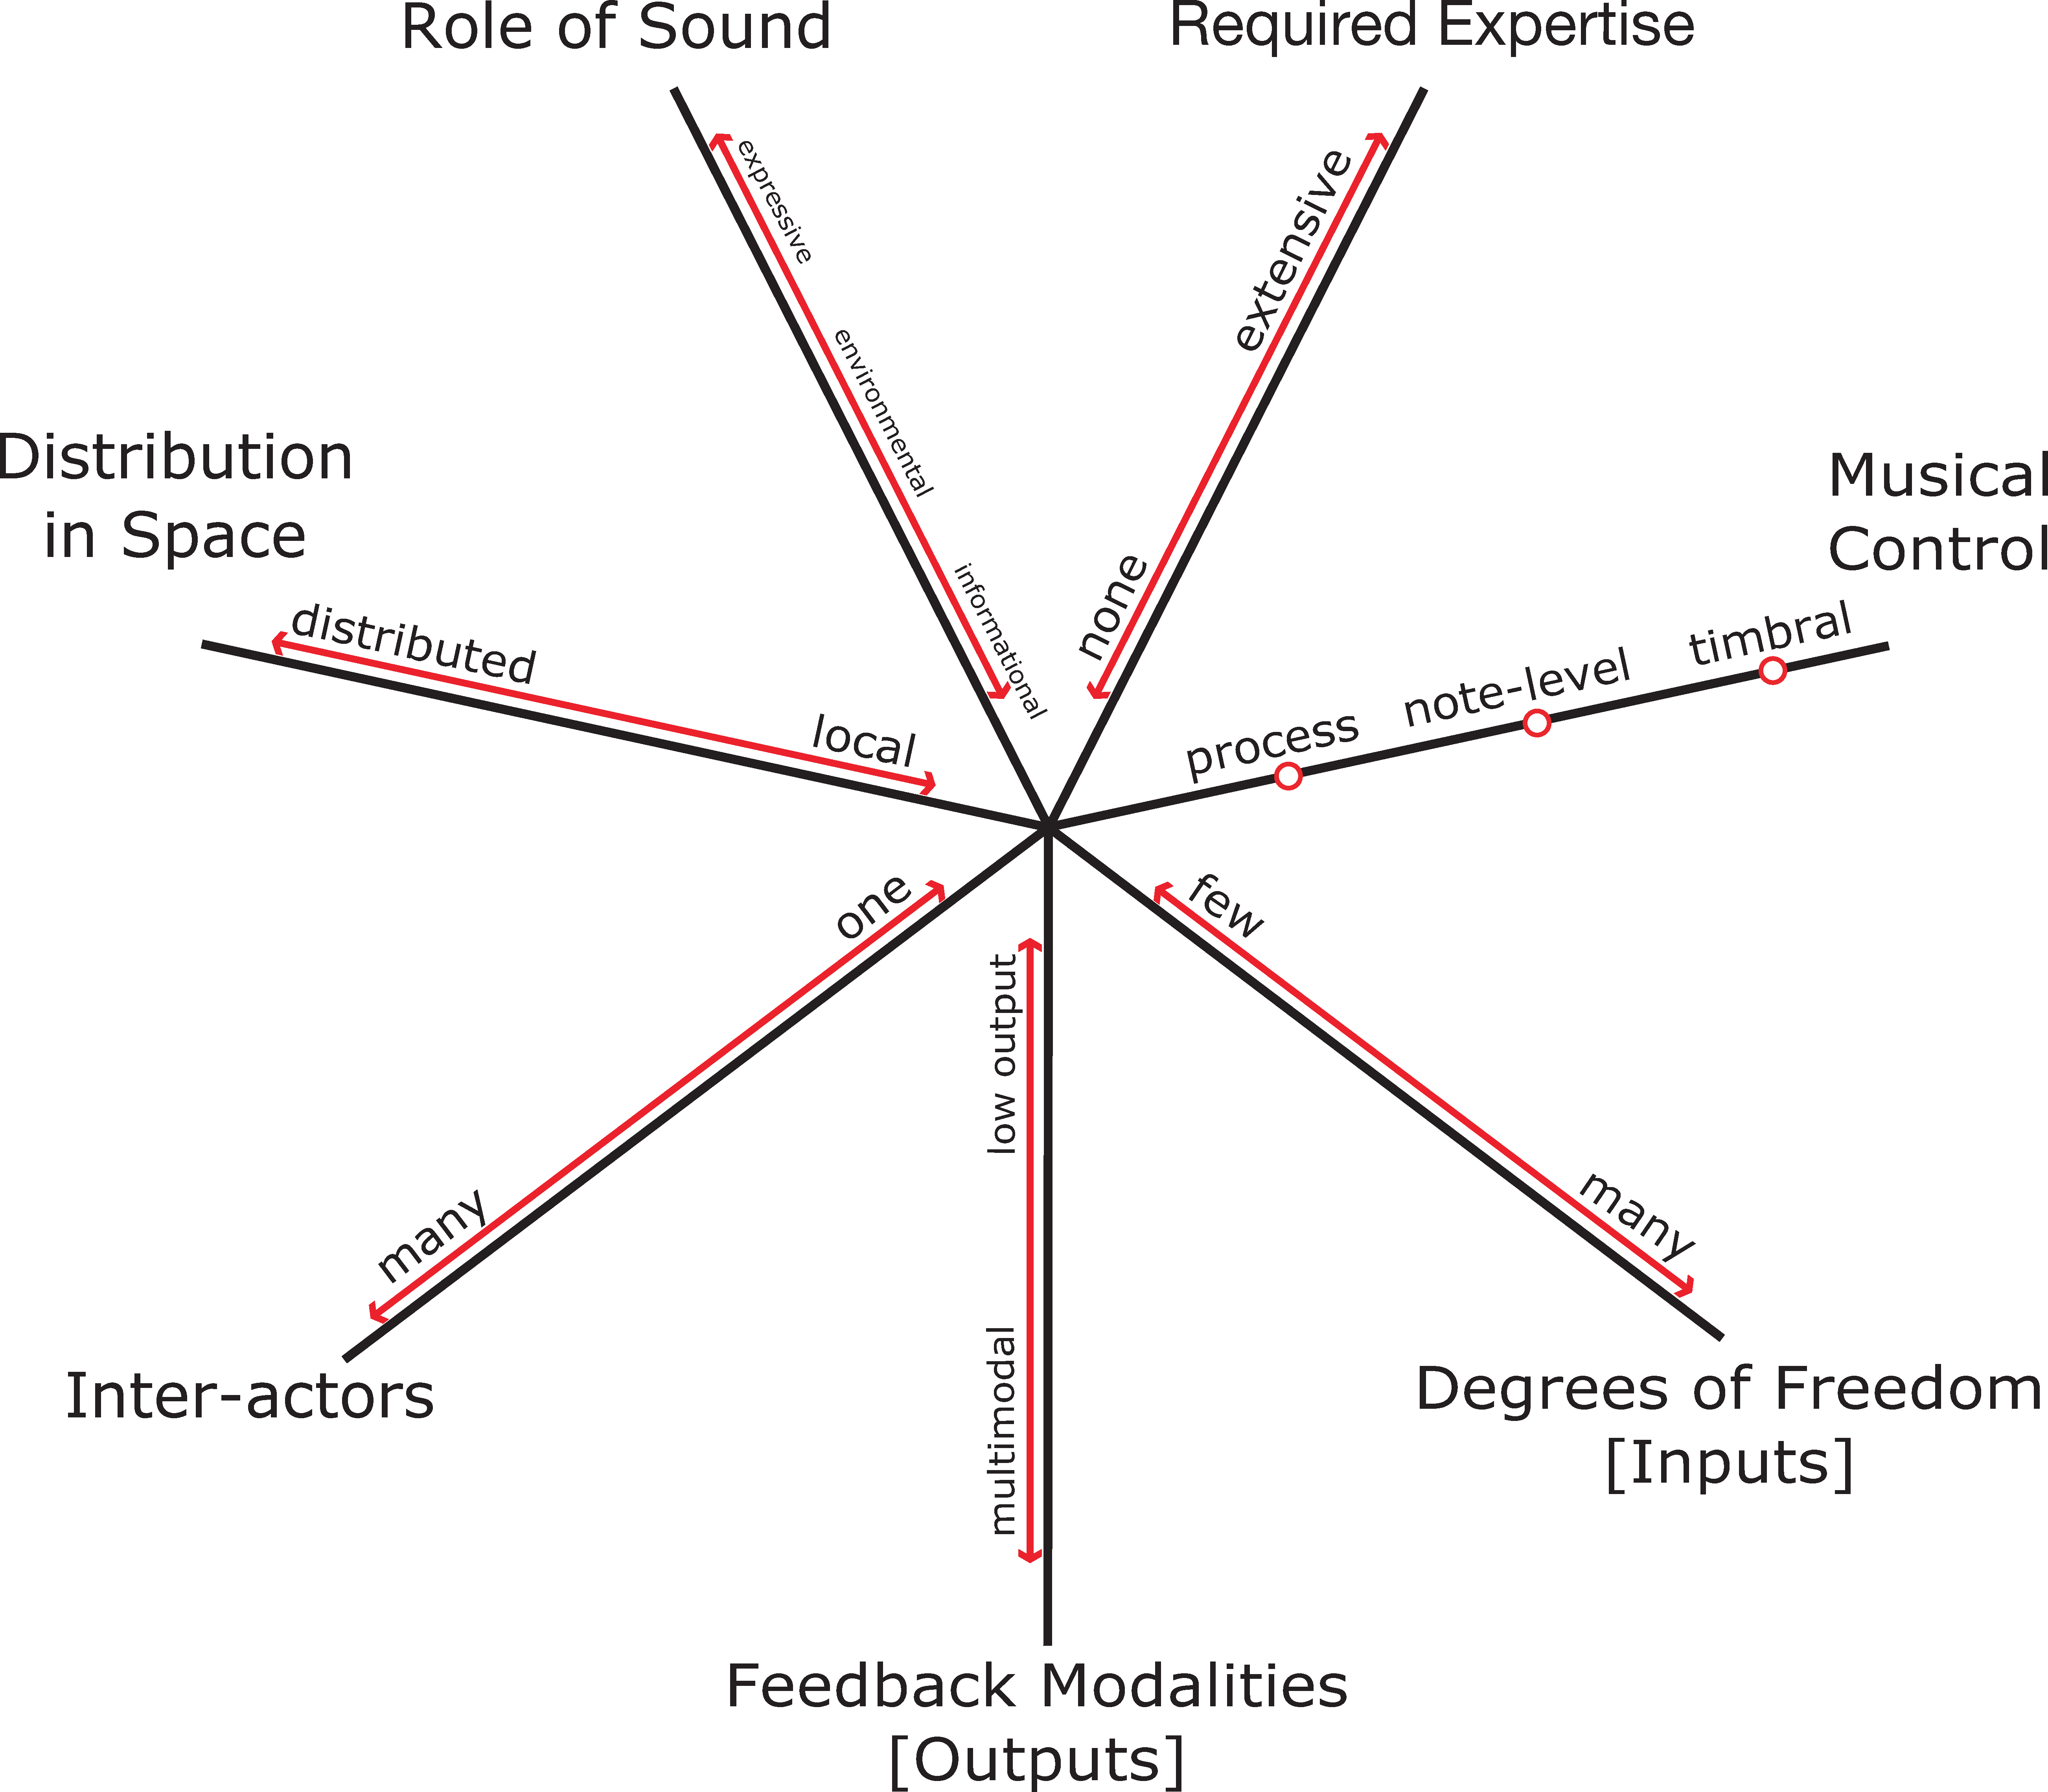
\includegraphics[width=\columnwidth]{figures/7axes}
\caption{The 7-axis Dimension Space}
\label{Birnbaum:fig:7axes}
\end{figure}

\begin{itemize}
	\item The \emph{Required Expertise} axis represents the level of practice and familiarity with the system that a user or performer should possess in order to interact as intended with the system. It is a continuous axis ranging in value from low to high expertise.
	\item The \emph{Musical Control} axis specifies the level of control a user exerts over the resulting musical output of the system. The axis is not continuous, rather it contains three discrete points following the characterization of \cite{Schloss:1990}, using three possible levels of control over musical processes: \emph{timbral level}, \emph{note level}, and \emph{control over a musical process}.
	\item The \emph{Feedback Modalities} axis indicates the degree to which a system provides real-time feedback to a user. Typical feedback modes include visual, auditory, tactile, and kinesthetic \cite{Wanderley:2000}.
	\item The \emph{Degrees of Freedom} axis indicates the number of input controls available to a user of a musical system. This axis is continuous, representing devices with few inputs at one extreme and those with many at the other extreme.
	\item The \emph{Inter-actors} axis represents the number of people involved in the musical interaction. Typically interactions with traditional musical instruments feature only one inter-actor, but some digital musical instruments and installations are designed as collaborative interfaces (see \cite{Fels:2002a,Blaine:2003a}), and a large installation may involve hundreds of people interacting with the system at once \cite{Ulyate:2001}.
	\item The \emph{Distribution in Space} axis represents the total physical area in which the interaction takes place, with values ranging from local to global distribution. Musical systems spanning several continents via the internet, such as Global String, are highly distributed \cite{Tanaka:2001a}.
	\item The \emph{Role of Sound} axis uses Pressing's \cite{Pressing:1997} categories of sound roles in electronic media. The axis ranges between three main possible values: \emph{artistic/expressive}, \emph{environmental}, and \emph{informational}.
\end{itemize}

\begin{figure}[ht]
%the following local setting was added to fix broken text justification
%width of subfigures increased from .4 to .47 so that captions fit on single line.
% mjl Feb. 27, 2016
\subcapraggedrighttrue
\centering
    \subfigure[\emph{The Hands} \cite{Waisvisz:1985}]
        {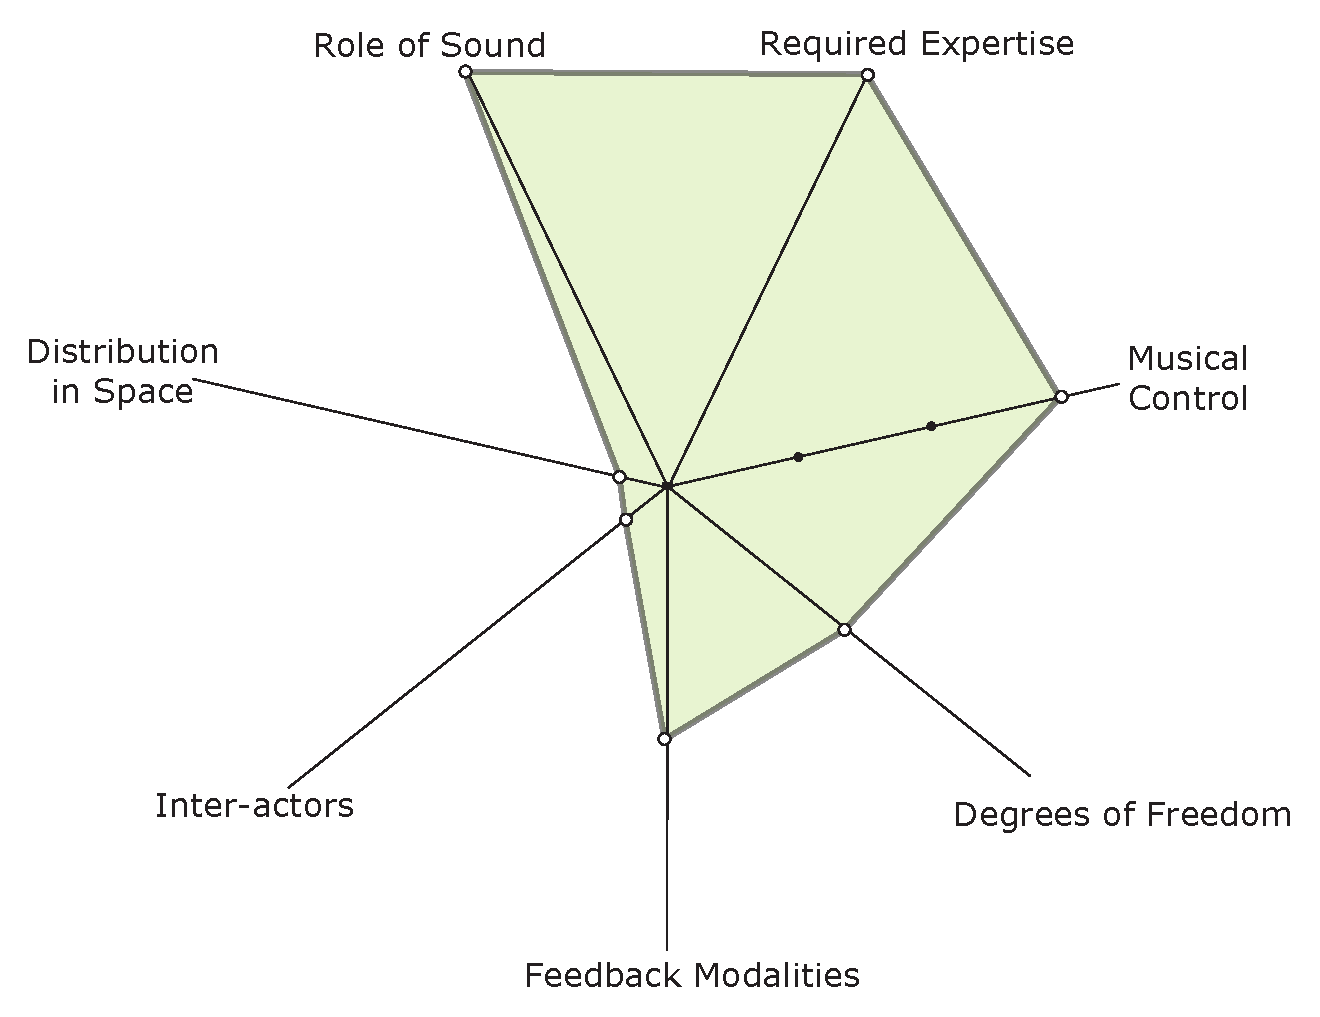
\includegraphics[keepaspectratio,width=0.47\columnwidth]{figures/the_hands}\label{Birnbaum:fig:hands}}
    \subfigure[\emph{Hyper-Flute} \cite{Palacio-Quintin:2003}]
        {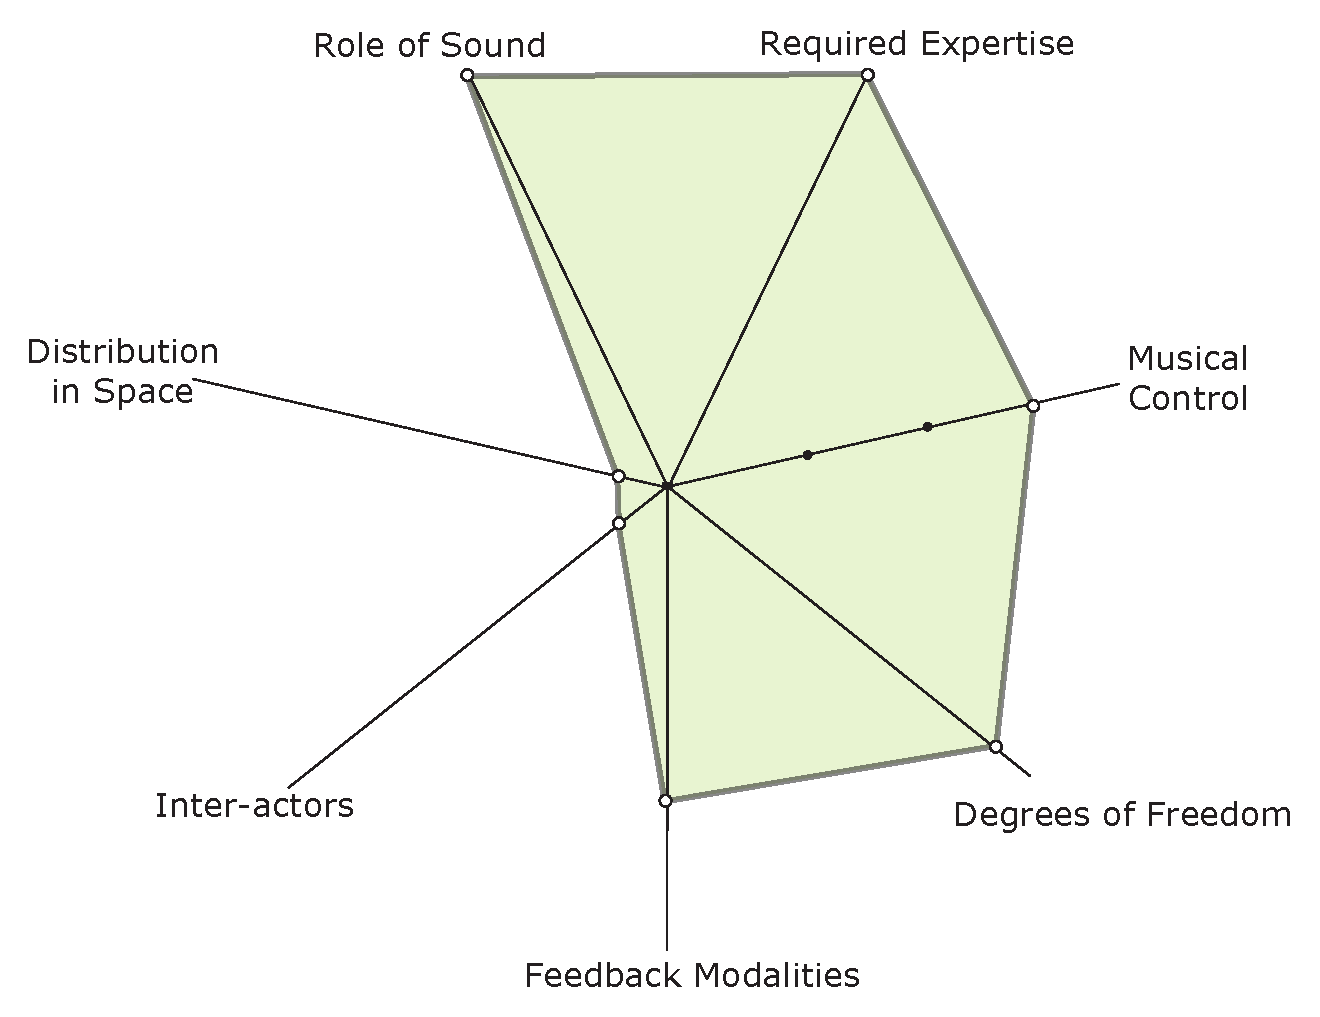
\includegraphics[keepaspectratio,width=0.47\columnwidth]{figures/hyper-flute}\label{Birnbaum:fig:hyper-flute}}
    \subfigure[Theremin]
        {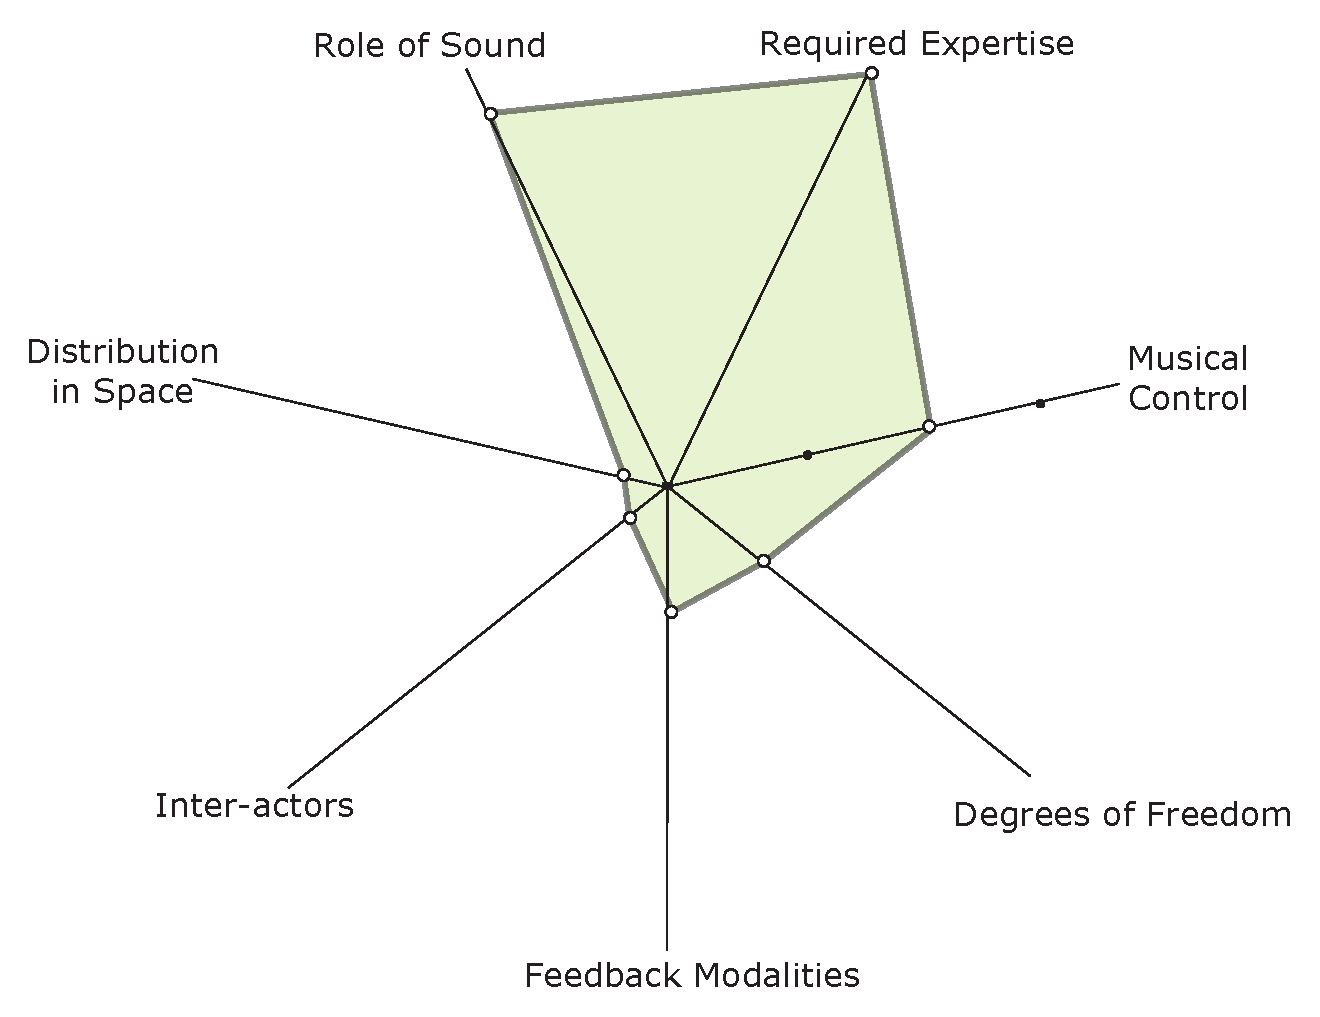
\includegraphics[keepaspectratio,width=0.47\columnwidth]{figures/theremin}\label{Birnbaum:fig:theremin}}
    \subfigure[\emph{Tooka} \cite{Fels:2002a}]
        {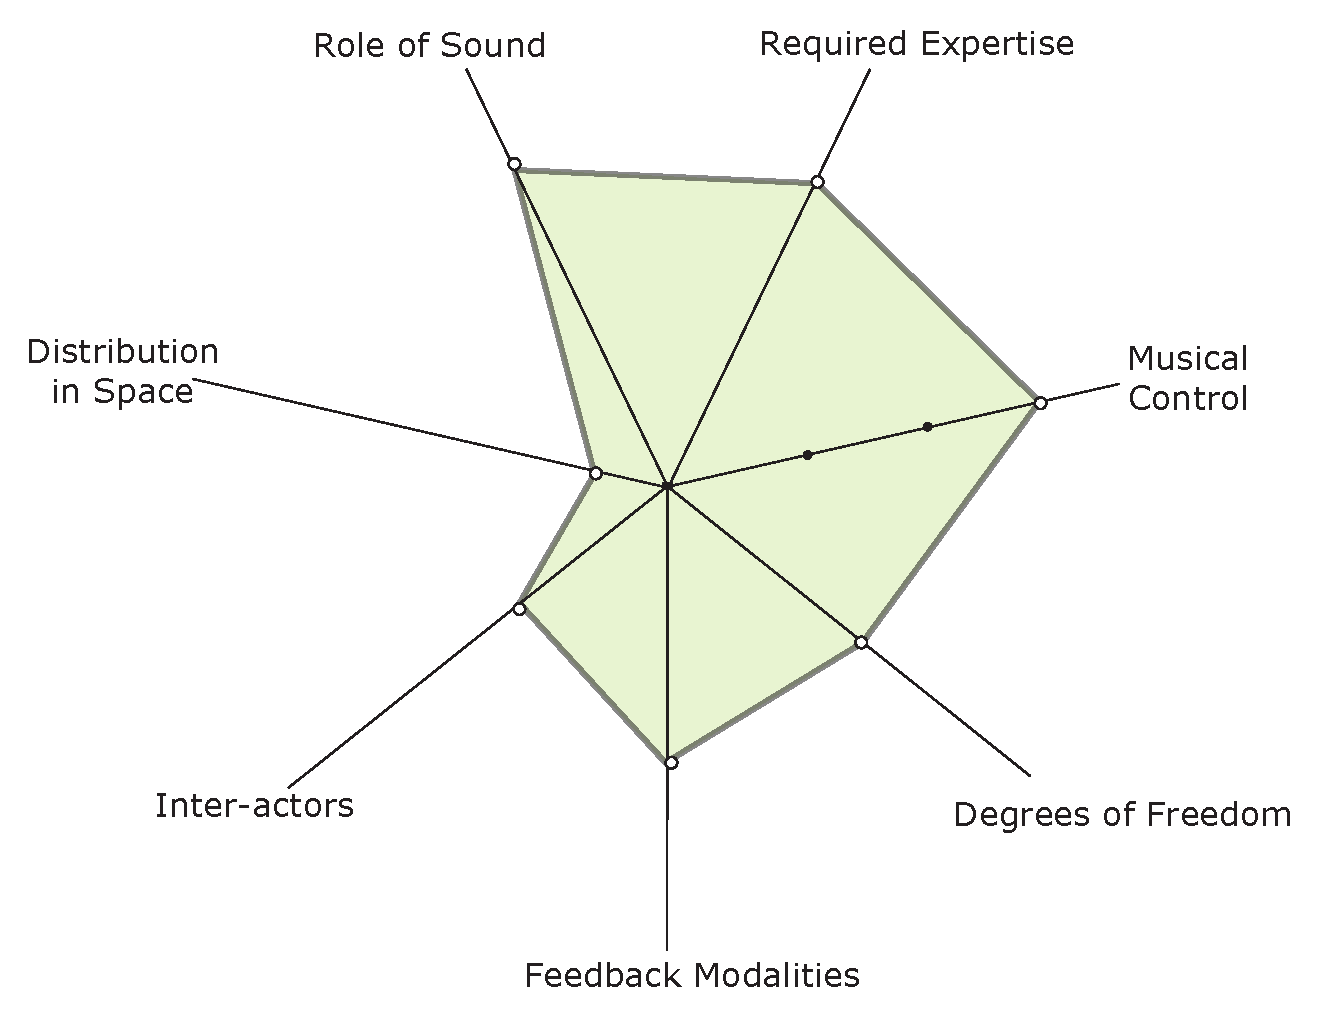
\includegraphics[keepaspectratio,width=0.47\columnwidth]{figures/tooka}\label{Birnbaum:fig:tooka}}
    \subfigure[\emph{Block Jam} \cite{Newton-Dunn:2003}]
        {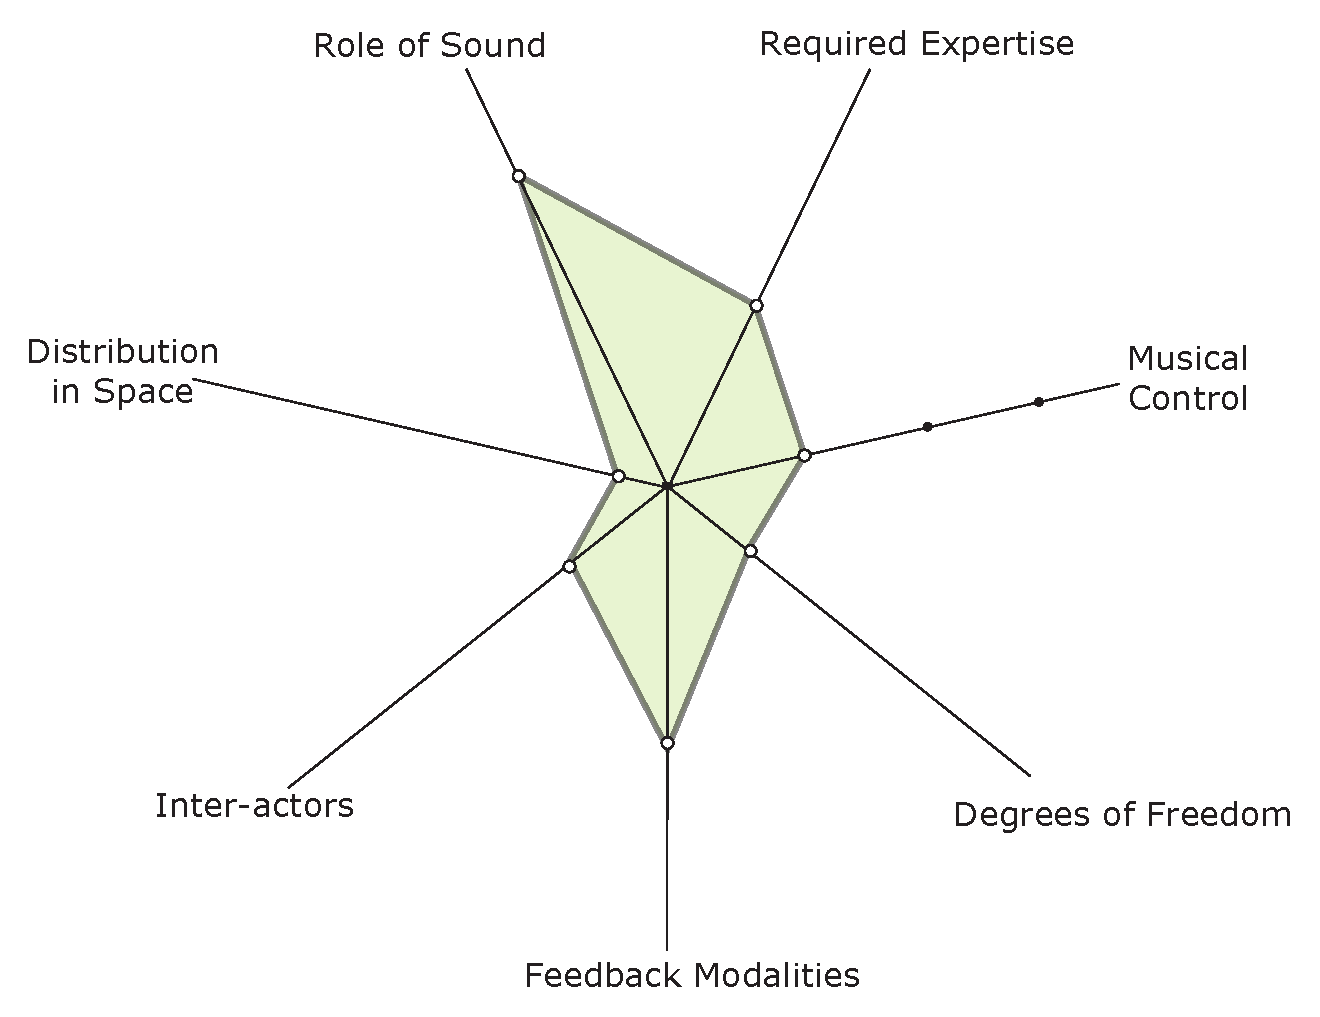
\includegraphics[keepaspectratio,width=0.47\columnwidth]{figures/block_jam}\label{Birnbaum:fig:block_jam}}
    \subfigure[\emph{Rhythm Tree} \cite{Paradiso:1999}]
        {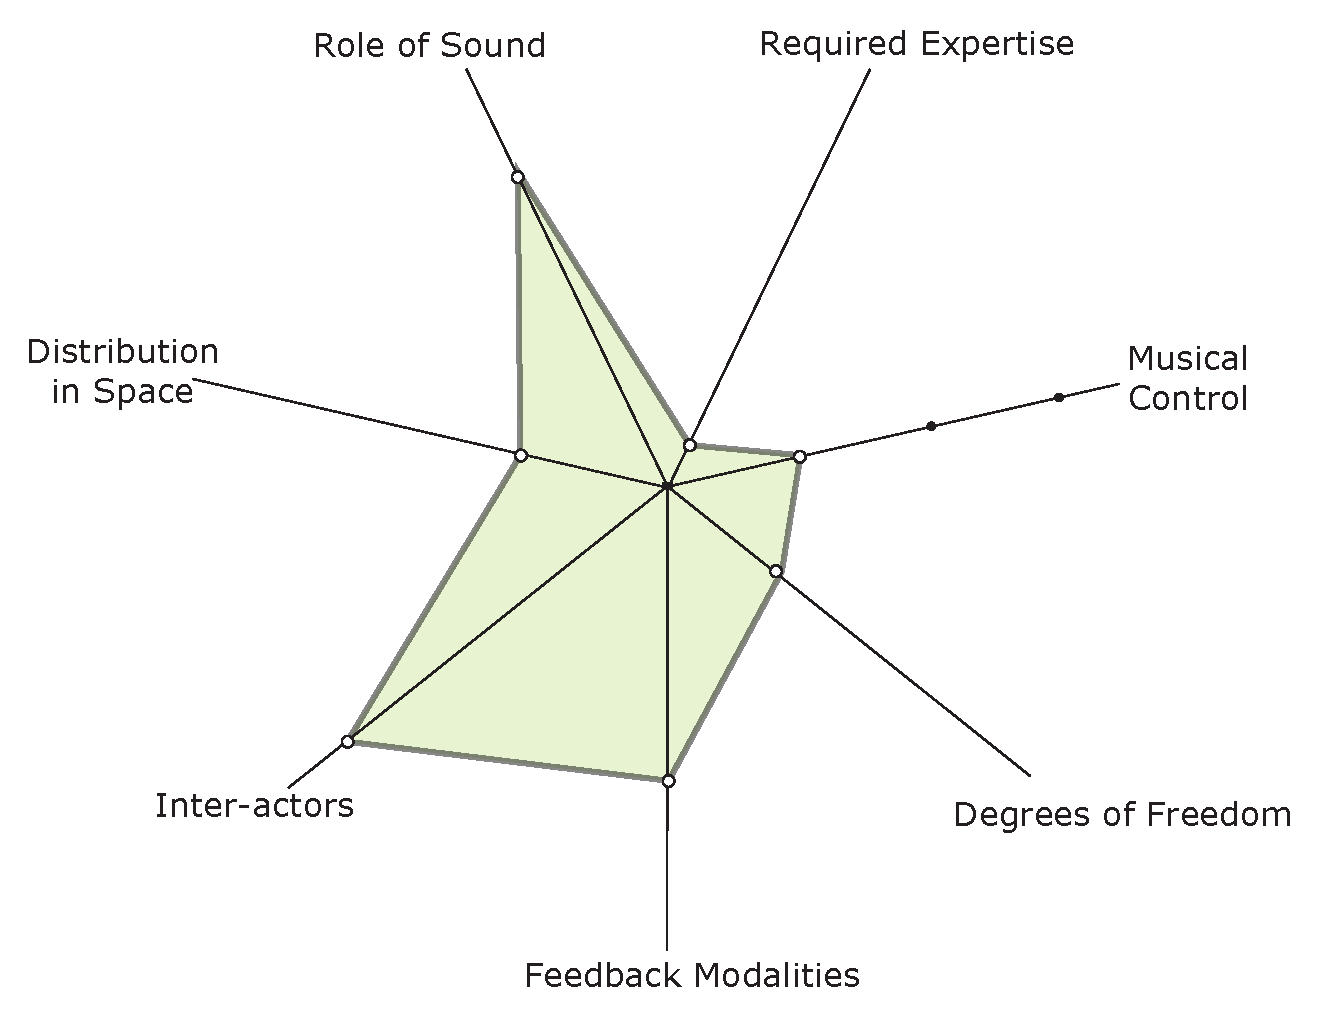
\includegraphics[keepaspectratio,width=0.47\columnwidth]{figures/rhythm_tree}\label{Birnbaum:fig:rhythm_tree}}
    \subfigure[\emph{Global String} \cite{Tanaka:2001a}]
        {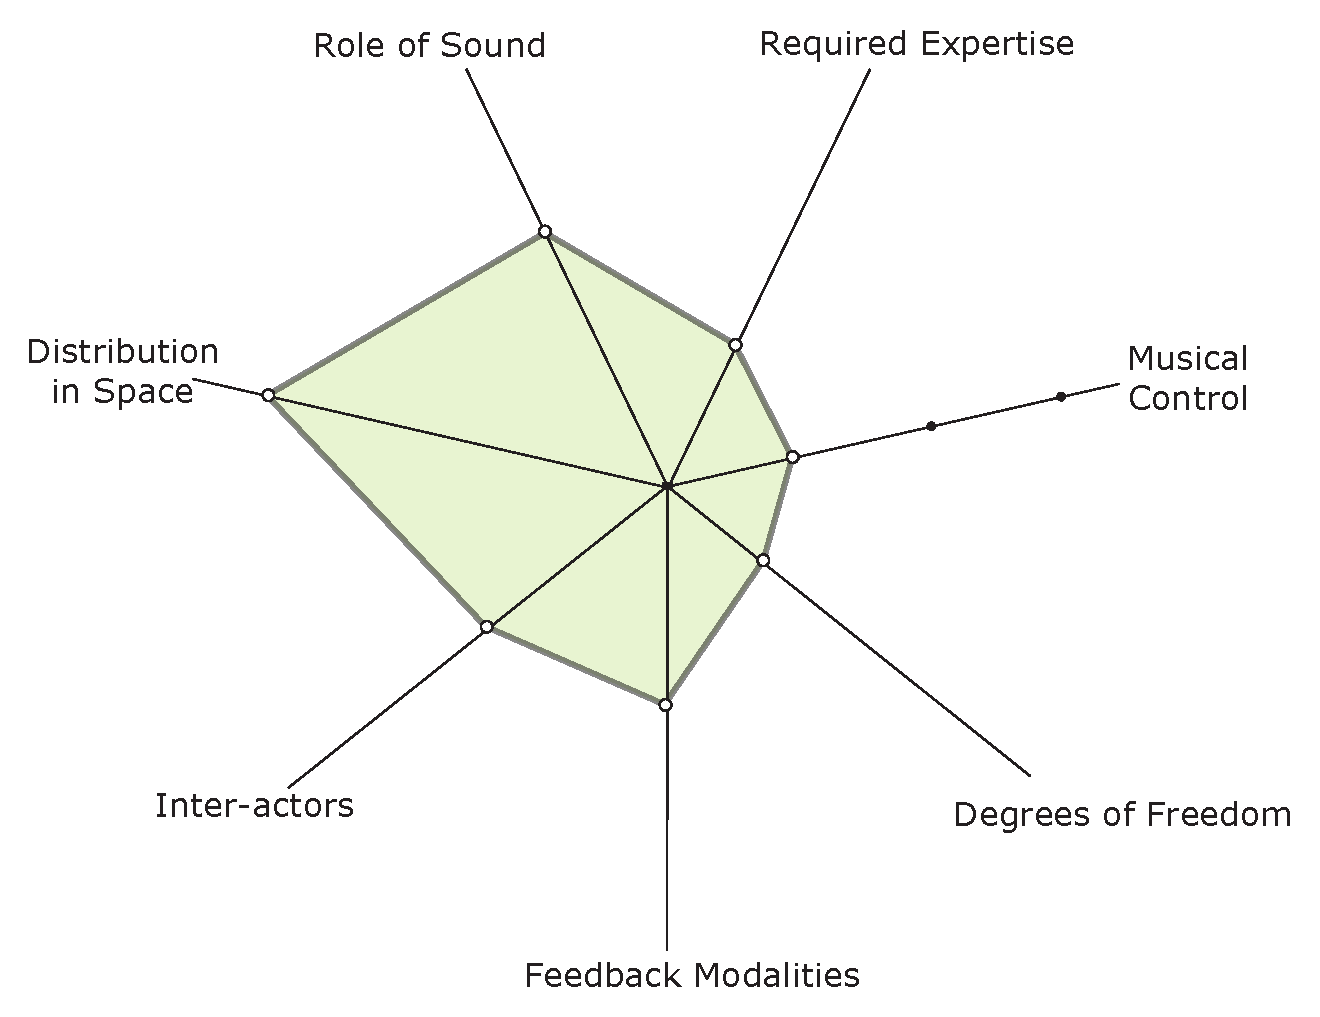
\includegraphics[keepaspectratio,width=0.47\columnwidth]{figures/global_string}\label{Birnbaum:fig:global_string}}
    \subfigure[\emph{Maybe...1910} \cite{Winkler:2000}]
        {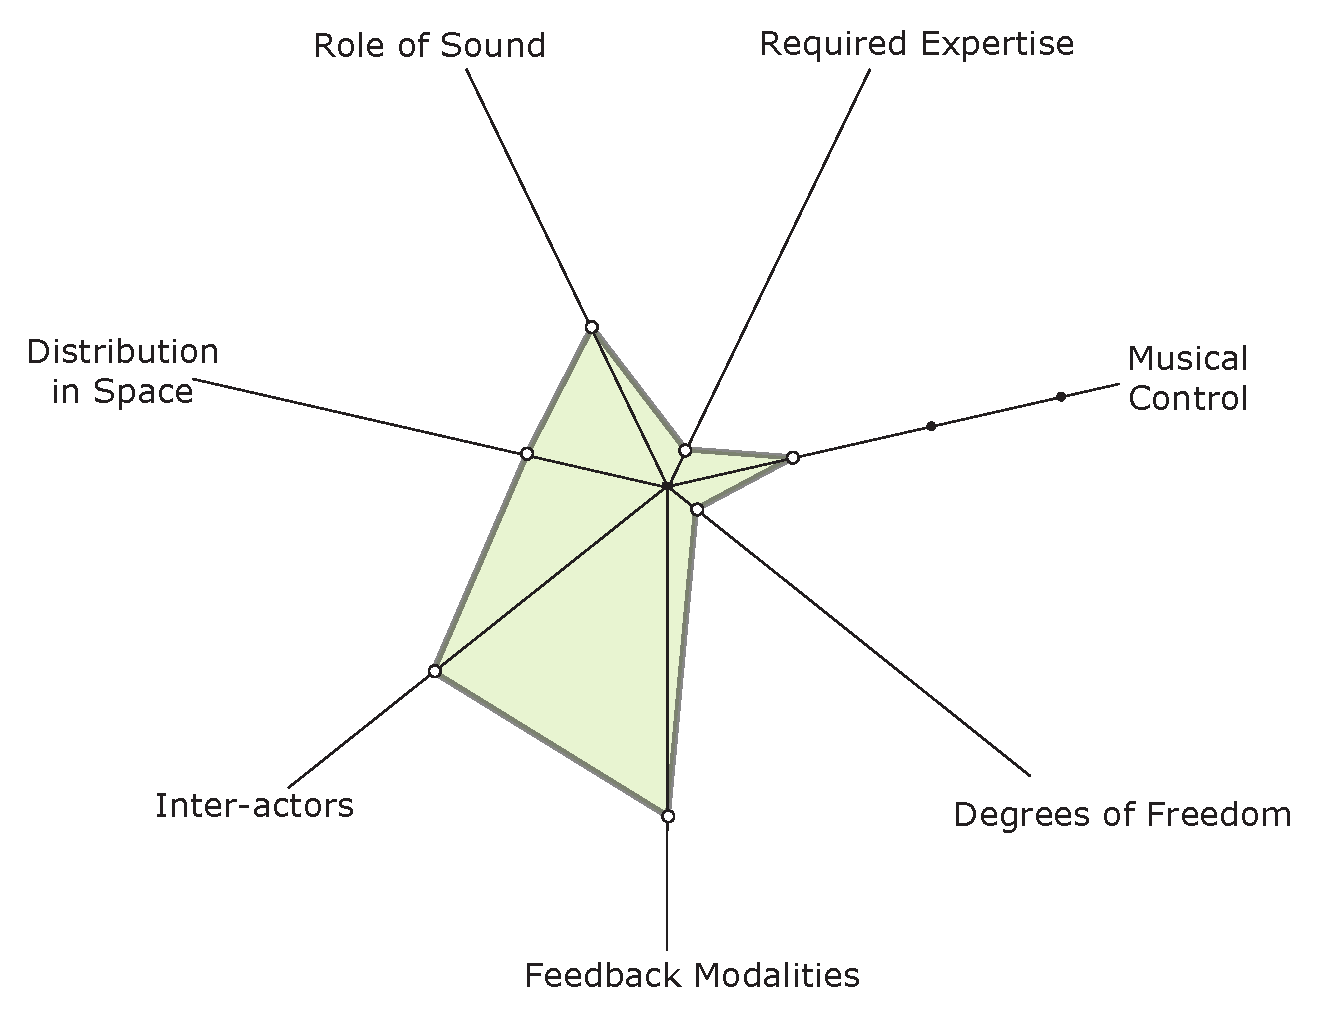
\includegraphics[keepaspectratio,width=0.47\columnwidth]{figures/maybe_1910}\label{Birnbaum:fig:maybe_1910}}
    \caption{Dimension Space Plots}
    \label{Birnbaum:fig:plots}
\end{figure}

\section{Trends in Dimension Plots}

The plots of Michel Waisvisz' \emph{The Hands} (Figure~\ref{Birnbaum:fig:hands}) and Todd Winkler's installation \emph{Maybe... 1910} (Figure~\ref{Birnbaum:fig:maybe_1910}) provide contrasting examples of the dimension space in use. \emph{The Hands} requires a high amount of user expertise, allows timbral control of sound (depending on the mapping used), and has a moderate number of inputs and outputs. The number of inter-actors is low (one), the distribution in space is local, and the role of the produced sound is expressive. The installation \emph{Maybe... 1910}, is very different: the required expertise and number of inputs are low, and only control of high-level musical processes (playback of sound files) is possible. The number of output modes is quite high (sights, sounds, textures, smells) as is the number of inter-actors. The distribution in space of the interaction, while still local, is larger than most instruments, and the role of sound is primarily the exploration of the installation environment.

When comparing these plots, and those of other music devices, it became apparent that the grouping used caused the plots of instruments to shift to the right side of the graph, and plots of installations to shift to the left. Installations commonly involve more people at the point of interaction, with the expectation that they are non-experts. Also, installations are often more distributed in space than instruments, which are intended to offer more control and a high potential for expressivity, achieved by offering more degrees of freedom. Sequencing tools, games, and toys typically occupy a smaller but still significant portion of the right side of the graph.

\section{Conclusions}

We have demonstrated that a dimension space paradigm allows visual representation of digital musical instruments, sound installations, and other variants of music devices. These dimension spaces are useful for clarifying the process of device development, as each relevant characteristic is defined and isolated. Furthermore, we found that the seven-axis dimension space resulted in visible trends between plots of related devices, with instrument-like devices tending to form one distinct shape and installations forming another shape. These trends can be used to present a geometric formulation of the relationships among existing systems, of benefit to device characterization and design.

Our future work in this direction might include further refinement of the system of axes, including changing the number of axes, or their definitions. Furthermore, a major problem remains insofar as the current plots are based partly on a subjective assessment of the devices. This assessment should be verified with empirical measurements from user tests \cite{Wanderley:2000}. Others who wish to employ dimension space analysis can adapt or change the axes as needed, though in the future a standard set of axes more universal in appeal may emerge.

\section*{Author Commentary: Dimension Spaces For Characterizing Musical Devices---A Reflection After Ten Years}

\paragraph{Joseph Malloch and Rebecca Fiebrink and David Birnbaum and Marcelo M. Wanderley}

Our work on characterizing new interfaces for musical expression dates back at least 15 years, to an article published by the last author with Nicola Orio and Norbert Schnell comparing interfaces from semantic (interaction) and system design (engineering) perspectives \cite{Wanderley:2000}. We were also aware of a number of other efforts, most notably the 2001 Diplomarbeit of J\"{o}rg Piringer which catalogues more than 100 instruments and devices and categorizes them based on immersiveness, expression, and output modalities \cite{Piringer:2001}.

This paper started as an exercise during the graduate seminar ``Gestural Control of Sound Synthesis'' at McGill University in Autumn 2004. (The first three authors were students in the seminar.) The aim of the exercise was to find a simple visual representation for comparing multiple properties of interfaces for musical expression, digital musical instruments, and interactive sound installations. Rather than trying to invent new metrics or descriptors, this representation would reflect the suggestions and judgements of the research field by relating and harmonizing taxonomies found in the existing literature.

For our representation we decided to adapt the ``dimension space'' approach used by Graham et al. to analyse interactive systems \cite{Graham:2000}. While Graham et al.'s work plotted each system from different perspectives and for different contexts, we used a single static dimension space mapped onto a radial plot to increase the ``glanceability'' of our visualizations. Starting with a list of 16 dimensions gleaned from the literature, we combined related dimensions wherever possible and slowly reduced the set to those most useful for differentiating real instruments, installations, and systems. Priority was given to properties that were less subject to individual interpretation, and axis names were chosen to avoid implication of value judgement.

With a more manageable space of system properties, we set to work informally evaluating different arrangements of axis ordering, polarity, and rotation for understandability, recognizability, and maximal differences in shape between system visualizations. For example, we tried to avoid configurations in which plots of real systems resembled ``stars'' since we determined that differences between star-shapes were not very legible without detailed investigation. Informal evaluations by colleagues also revealed a common misreading of the six-axis plots as used by Graham et al. as depictions of three-dimensional space rather than radial dimension spaces---to avoid this we adjusted our own spaces to either use an odd number of dimensions or rotate the space so that none of the axes were vertical.

The number of citations received by the paper indicates widespread interest for a fairly small research community. Several more design spaces for musical interfaces have also been suggested, but there is still no generally accepted set of properties for comparing or categorizing music interfaces. The most recent major work we are aware of in this direction is the TIEM project,\footnote{\url{http://vipre.uws.edu.au/tiem/}} led by Garth Paine and Jon Drummond, and with the collaboration of music technology veterans such as Joel Chadabe (a pioneer of interactive systems), Axel Mulder (Infusion Systems, who developed seminal work in the field during the 1990s), and the last author of this paper. TIEM involves both a detailed survey of existing musical instruments and a public catalogue of contributed instruments and interfaces.

Finally, to celebrate the tenth anniversary of the original publication, we have embedded an interactive version of the dimension space on the IDMIL website.\footnote{\url{http://idmil.org/projects/interface_evaluation/dimension_space}} It allows visitors to see and compare the plots of more than 170 interfaces, and to search the database simply by drawing a dimension space.

We hope this paper will continue to be useful for other works proposing improved ways to compare musical devices and systems (e.g., \cite{Morreale:2014,Malloch:2006}). Shedding light into their similarities and differences is a promising way to achieve more developed designs and eventually more rewarding musical instruments and systems.


\section*{Expert Commentary: Towards Many Dimension Spaces for Musical Devices}

\paragraph{Florent Berthaut}

In this paper, the authors propose a novel approach for dealing with two essential questions in the field of New Interfaces for Musical Expression (NIME). The first is that of evaluation: how does one characterize and measure the properties of a musical interface, in order to assess how well it fulfils certain goals and/or compare it with other interfaces? This issue has previously been tackled in different ways, such as defining a formula  for ``efficiency'' of an instrument \cite{Jorda:2003}, or by adapting methods from Human Computer Interaction (HCI) for comparing performance on specific musical tasks \cite{Orio:2002}. While these approaches offer valuable results, they remain limited in that they impose fixed objectives, whereas actually these objectives may vary due to the very subjective nature of the output, which can depend on context and on the listeners. The current article provides a method enabling a more flexible evaluation of NIMEs. The second question is that of design guidelines: how does one design a musical interface to fulfill specific objectives? Instead of providing a fixed set of rules, the approach presented by the authors enables an incremental and comparative approach to the design of novel musical interfaces.

In their paper, the authors propose the use of \emph{dimension space analysis}, a method for the visual analysis of systems relying on the notion that all interfaces inhabit a design space defined by a finite set of properties \cite{Graham:2000}. Each property is represented using an axis running from the centre point of the graph towards the vertices of a 2D shape. This resulting shape, which depends on the choice and configuration of the axes, allows visual comparison of systems with respect to the design space. Dimension Spaces also permit the evaluation of system tendencies that appear as particular spatial configurations.

In my opinion, the article offers two main contributions. The first is the proposal to use dimension space analysis for understanding and designing musical interfaces. The method appears to be extremely relevant in a field where evaluation criteria depend strongly on the context in which the interface is both used and perceived. Changing the axes and their spatial arrangement allows for easy experimentation with various analyses and comparisons. The article therefore encourages other researchers to create dimension spaces reflecting their own specific analysis needs,  for example, by focusing on the scenographic aspect of musical interfaces as was done in \cite{Berthaut:2014}. For the design of new interfaces, dimension spaces frees one from relying on a fixed set of rules, and encourages the exploration of transformations of existing interfaces, e.g. ``how can we increase the property X of this interface'' or ``what would this interface become with a shift in all its axes.'' This could make the design of new musical interfaces more accessible. The second main contribution of the article is the ``seven axes Dimension Space'' proposed by the authors. While it is provided as an example, it actually constitutes a set of essential properties that have emerged in a number of previous research works on NIMEs. This dimension space is well-suited for distinguishing between installations and instruments, i.e. between interfaces oriented towards novices and those oriented towards experts. It was therefore perfectly suited for  the evaluation of an instrument having multiple levels of expertise \cite{Berthaut:2010}.

I agree with the authors' observation that the subjective axes chosen could be complemented with properties from user studies measurements, and that this constitutes an interesting future work. I would however disagree with the last sentence of the paper, regarding a standard set of axes with which all musical interfaces could be evaluated. In my opinion, an exciting alternative perspective on this work can be gained by considering an extensible and publicly shared set of axes, which could be  created and refined collaboratively via an online platform. I believe that new perspectives would arise for the evaluation and comparison of musical interfaces by allowing researchers to: (a) add new axes and properties, (b) discuss the evaluation and measurement of these axes, (c) insert and evaluate new interfaces along the axes, and (d) create dimension spaces from subsets of the axes. Another result of such an approach would be the chronological study of how interfaces evolve regarding specific axes and properties. It could in the long run also allow studies of the potential evolution of the axes themselves, reflecting the changes in priorities and expectations of ``NIMErs.''

